\documentclass[12pt, titlepage]{article}
\usepackage{polski}
\usepackage[utf8]{inputenc}
\usepackage{amsmath}
\usepackage{amsfonts}
\usepackage{multirow}
\usepackage{graphicx}
\usepackage{caption}
\usepackage{subcaption}
\usepackage{hyperref}


\begin{document}
\begin{titlepage}

\newcommand{\HRule}{\rule{\linewidth}{0.5mm}} % Defines a new command for the horizontal lines, change thickness here

\center 

\textsc{\LARGE Politechnika Śląska}\\[1.2cm] 

\textsc{\Large Wydział Matematyki Stosowanej}\\ 
\textsc{\Large Informatyka, sem. VI}\\[0.8cm]

\textsc{\large Aplikacje bazodanowe}\\
\textsc{\large Dokumentacja Projektu}\\[0.7cm] 


\HRule \\[0.7cm]
{ \huge \bfseries eRegistry}\\[0.4cm] 
\HRule \\[0.7cm]
 
\begin{minipage}{0.8\textwidth}
\begin{flushleft} \large
\emph{Autorzy:}\\
Karolina \textsc{Chrząszcz}\\
Szymon \textsc{Górnioczek}\\
Wiktor \textsc{Gruszczyński}\\
Jarosław \textsc{Kania}\\
Tomasz \textsc{Kryg}\\
\end{flushleft}

\begin{flushright}
\href{http://github.com/szymongor/eRegistry}{Repozytorium}
\end{flushright} \large

\end{minipage}\\[0.7cm]


\includegraphics[scale=0.5]{img/logo.jpg}\\[1cm]
{\large \today}\\[0.5cm] 

\vfill % Fill the rest of the page with whitespace

\end{titlepage}

\tableofcontents

\newpage

\section{Temat projektu}
Naszym zadaniem jest stworzenie elektronicznego dziennika szkolnego. Dziennik ten powinien umożliwić, uczniom i ich opiekunom, wgląd do ocen ucznia z przedmiotów, na które uczęszcza oraz dać możliwość nauczycielom wprowadzania tych ocen. 

Dzięki projektowi rodzice na bieżąco będą mieli wgląd w szkolne życie swoich dzieci oraz ułatwi to komunikację z nauczycielami.   

\section{Opis ogólny wymagań}

Na podstawie przeprowadzonej analizy zagadnienia przygotowaliśmy listę podstawowych funkcjonalności, którą powinien realizować nasz projekt.

Każda osoba, mająca dostęp do dziennik, będzie nazywana użytkownikiem. Każdy użytkownik będzie miał stworzone własne konto, dzięki któremu będzie miał wgląd do odpowiednich zasobów dziennika. Zostanie mu również przypisana \textit{data ważności} (data, po której powinien zostać usunięty dostęp do dziennika) oraz informacja o tym, czy jest \textit{aktywnym} użytkownikiem.

W trakcie tworzenia konta, administrator wprowadzi dane osobowe użytkownika oraz przydzieli mu odpowiednie uprawnienia. Po zalogowaniu się, użytkownicy poza wyświetleniem odpowiednich informacji będą mogli edytować swoje dane, oraz zmienić hasło. W celu ułatwienia opisu funkcjonalności podzieliliśmy użytkowników na podane niżej grupy:

\subsection{Uczniowie}

Każdy uczeń posiadający konto, powinien mieć wgląd do swoich ocen, przedmiotów na które uczęszcza, informacji o sobie, prowadzących zajęcia oraz klasy do której należy.

Oceny będą dzielić się na:
\begin{itemize}
\item ocena częściowa -- pomniejsza ocena związana z pewną aktywnością ucznia na zajęciach. Może to być ocena za sprawdzian, odpowiedź lub zadanie domowe. Oprócz otrzymanego stopnia będzie wyświetlona waga oceny, informacja za co została wystawiona oraz data wystawienia.
\item ocena semestralna -- ocena podsumowująca pracę ucznia przez cały semestr. Jest ona wyliczana na podstawie ocen częściowych ucznia, osobno dla każdego przedmiotu.
\item ocena końcowa -- główna ocena wystawiana z każdego przedmiotu po całym roku zajęć. Jest to średnia z dwóch ocen semestralnych: za pierwszy oraz za drugi semestr.
\end{itemize}

Uczeń z przedmiotu, jako ocenę końcową, może uzyskać między innymi ocenę niedostateczną. Oznacza ona, że nie uzyskuje on promocji do następnej klasy. W takim wypadku zostaje on  przepisany do innej klasy (rok wcześniej) i kontynuuje swoją naukę w tej klasie.

Uczniowie należą do klas. Klasa posiada swój profil oraz wychowawcę. Między klasami z tego samego rocznika mogą występować grupy. Grupa jest to większa ilość uczniów uczestniczących razem w konkretnych zajęciach. Jedna klasa może się dzielić na grupy (na przykład w $IIIa$ mogą być dwie grupy z języka angielskiego różniące się między sobą poziomem zaawansowania) lub jedna grupa może łączyć w sobie osoby z różnych klas (na przykład dziewczyny z $IIIa$ i $IIIb$ mogą razem uczęszczać na zajęcia z wychowania fizycznego).  

W przypadku uczniów \textit{data ważności} będzie rozumiana jako przewidywana data końca jego edukacji w konkretnej placówce (w przypadku nieotrzymania promocji do następnej klasy, data ta zostanie przedłużona o rok).

\subsection{Opiekun}

Z perspektywy uprawnień i funkcjonalności, opiekun jest prawie takim samym użytkownikiem, co uczeń. Jedyna różnica polega na tym, że po zalogowaniu zostaje wyświetlona lista uczniów, którymi się opiekuje. Po wyborze swojego dziecka zostaną wyświetlone takie same informacje, co uczniowi (zajęcia z ich prowadzącymi na, które uczęszcza dziecko i jego oceny wraz z ich opisem).
Opiekun ma również możliwość edycji danych osobowych swojego podopiecznego.

\textit{Data ważności} w przypadku opiekuna to przewidywana data końca nauki jego podopiecznego (w przypadku kilku podopiecznych zostanie wzięta pod uwagę bardziej odległa data). 

\subsection{Nauczyciel}

Osobą pełniącą główną pieczę nad ocenami jest nauczyciel. Może być przypisany do każdej z klas jako jej wychowawca. Dodatkowo każdy z nauczycieli prowadzi zajęcia z pewnego przedmiotu. 
Po zalogowaniu na swoje konto, powinien móc wyświetlić wszystkie grupy, w których prowadzi zajęcia. Po wyborze konkretnej grupy, zostanie wyświetlona lista uczniów należących do niej oraz oceny, jakie do tej pory im wystawił.

Po wybraniu konkretnego ucznia nauczyciel będzie mógł edytować dotychczasowe oceny oraz dodawać nowe (wraz z odpowiednim opisem - legendą, wagą i datą). Nauczyciel samodzielnie wystawia każdą z ocen, na podstawie osiągnięć uczniów z danego przedmiotu.

W przypadku nauczyciela, \textit{data ważności} rozumiana jest, jako data końca umowy. W przypadku przedłużenia umowy, data ulega zmianie. W przypadku dłuższego urlopu lub braku prowadzonych zajęć w danym semestrze, użytkownik będzie oznaczony jako \textit{nieaktywny}.

\subsection{Wybór technologii}

Na podstawie powyższej analizy postanowiliśmy napisać osobną aplikację dla nauczycieli i uczniów - aplikacja na urządzenia mobilne z systemem Android. Natomiast panel administratorski i nauczycielski postanowiliśmy zrealizować w wersji webowej. 
Dla wszystkich użytkowników połączenie z internetem będzie koniecznym warunkiem korzystania z dziennika.

\section{Aplikacja na Androida dla opiekuna i ucznia}

Aplikacja kliencka jest napisana w androidzie aby umożliwić swobodny dostęp do danych. Aplikacja kierowana dla uczniów oraz ich opiekunów dlatego wymagania rozpisano dla obu grup.

\subsection{Wymagania ogólne}

\begin{enumerate}
 \item Możliwość zalogowania (zapamiętaj login/hasło).
 \item Możliwość zmiany hasła (trzeba ustawić przy pierwszym. uruchomieniu, hasło generowane przy tworzeniu użytkownika).
 \item Obliczanie średniej ważonej (Wyświetla na kafelku przedmiotu).
 \item Wyświetlanie przedmiotu, ocen cząstkowych z datami. wystawienia
 \item Zmiana danych (mail, telefon).
\end{enumerate}

\subsubsection{Funkcjonalności opiekuna}

\begin{enumerate}
\item Wybór podopiecznego dla którego wyświetlać oceny.
\item Zmiana adresu zamieszkania opiekuna oraz podopiecznych. (zastosuj dla podopiecznych).
\item Wyświetlanie danych wychowawcy, możliwość wykonania połączenia z poziomu aplikacji.
\end{enumerate}


\subsubsection{Funkcjonalności opcjonalne}

\begin{enumerate}
\item Oznaczenie o nowych ocenach od ostatniego logowania.
\item W zależności od płci podopiecznego w menu wyboru odpowiednia \\ ikona.
\item W dniu urodzin życzenia.
\item Wyświetlanie pomocy.
\end{enumerate}


\subsection{Opis interfejsu}

Po uruchomieniu aplikacji ukaże się ekran logowania. Po zalogowaniu użytkownik zostanie przeniesiony do menu głównego z którego można nawigować do poszczególnych funkcjonalności.

\subsection{Uwagi}

\begin{enumerate}
\item Podwójne kliknięcie wstecz w menu głównym wychodzi z aplikacji (po pierwszym kliknięciu 'toast' z informacją o tym)

\item Opiekun może tylko wyświetlić mail oraz nr. telefonu podopiecznego. może edytować jego adres zamieszkania.

\item Uczeń nie może edytować miejsca zamieszkania, może edytować mail oraz nr. telefonu.

\item Na kafelku wyboru przedmiotu wyświetla się aktualna średnia ważona przedmiotu. (Może w zależności od stopnia zmieniać kolor)
\end{enumerate}



\begin{figure}
\centering
\begin{minipage}{.5\textwidth}
  \centering
  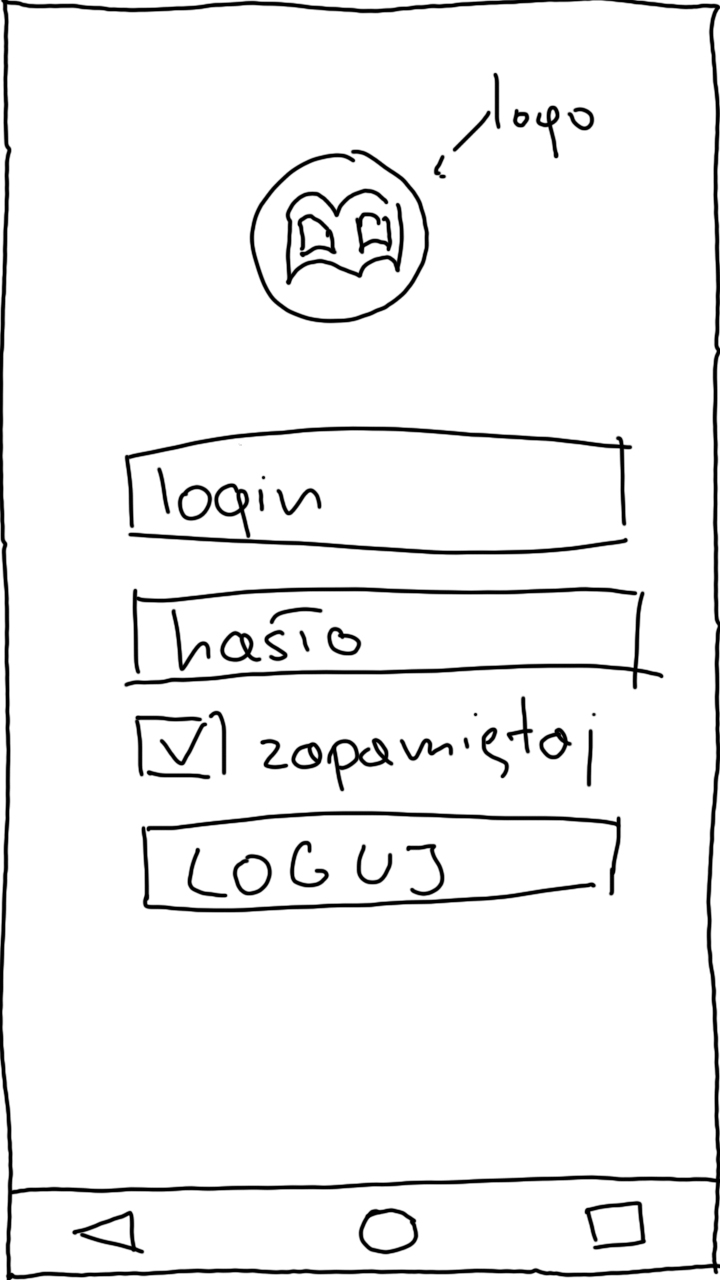
\includegraphics[width=.4\linewidth]{AplikacjaAndroid/Interfejs/EkranLogowania.jpg}
  \captionof{figure}{Ekran logowania}
  \label{fig:test1}
\end{minipage}%
\begin{minipage}{.5\textwidth}
  \centering
  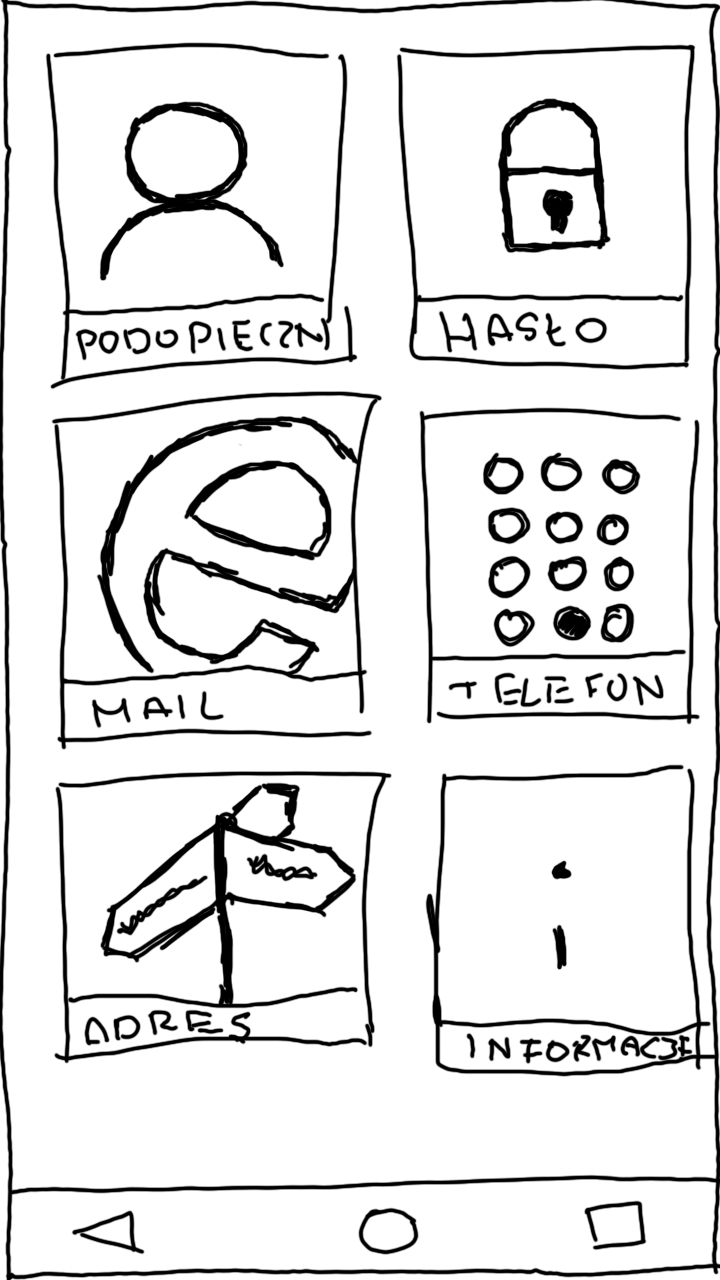
\includegraphics[width=.4\linewidth]{AplikacjaAndroid/Interfejs/Menu1.jpg}
  \captionof{figure}{Menu główne \\ (dla opiekuna)}
  \label{fig:test2}
\end{minipage}
\end{figure}

\begin{figure}
\centering
\begin{minipage}{.5\textwidth}
  \centering
  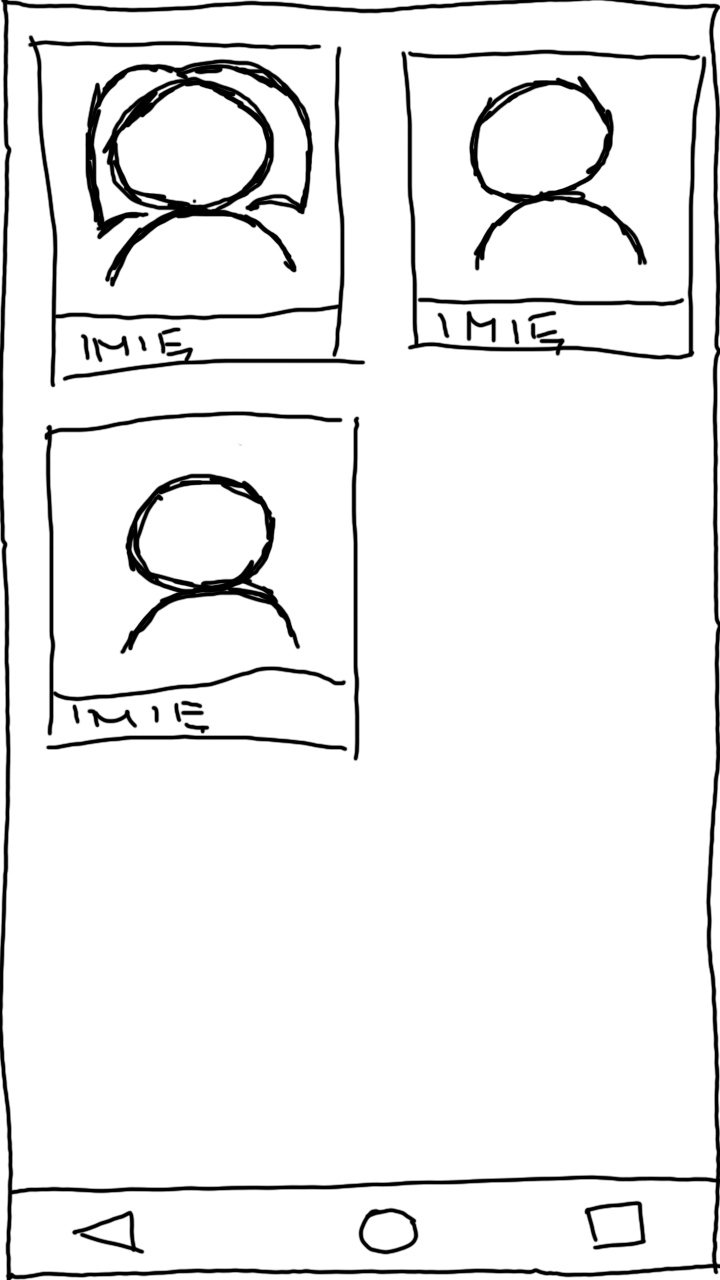
\includegraphics[width=.4\linewidth]{AplikacjaAndroid/Interfejs/Menu2.jpg}
  \captionof{figure}{Wybór podopiecznego\\ (dla opiekuna)}
  \label{fig:test1}
\end{minipage}%
\begin{minipage}{.5\textwidth}
  \centering
  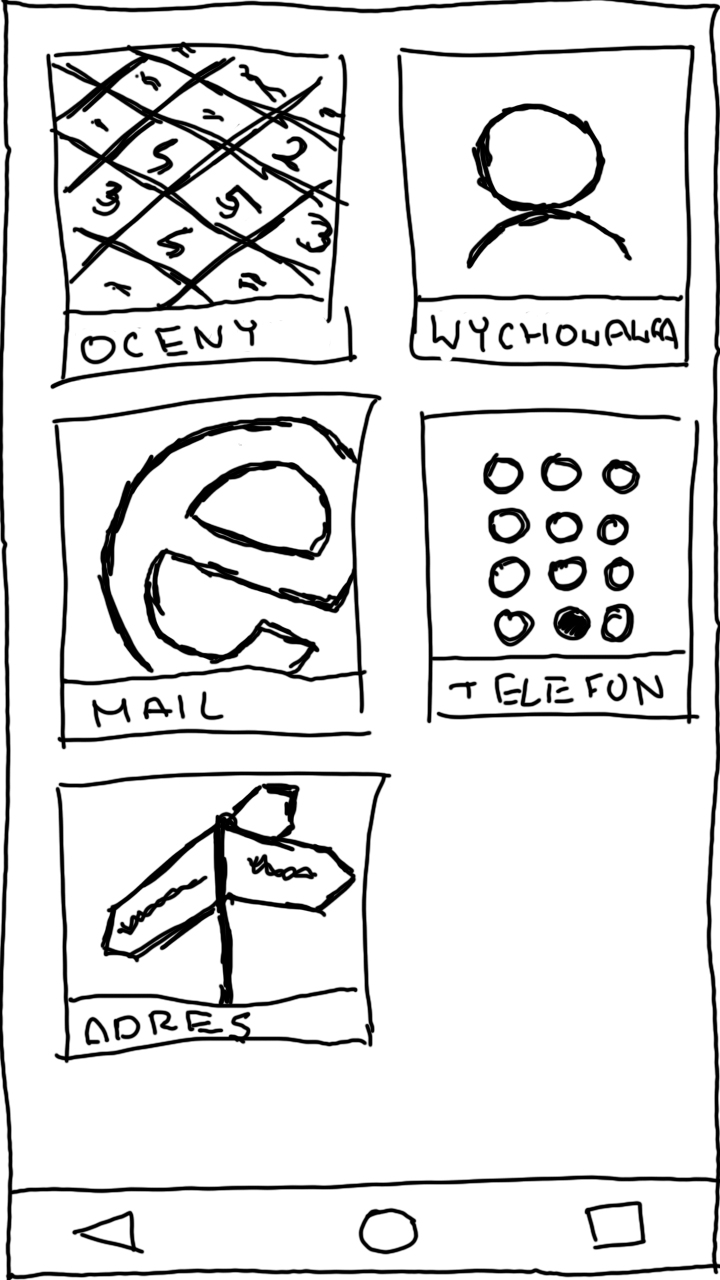
\includegraphics[width=.4\linewidth]{AplikacjaAndroid/Interfejs/Menu3.jpg}
  \captionof{figure}{Menu główne (dla ucznia)}
  \label{fig:test2}
\end{minipage}
\end{figure}


\begin{figure}
\centering
\begin{minipage}{.5\textwidth}
  \centering
  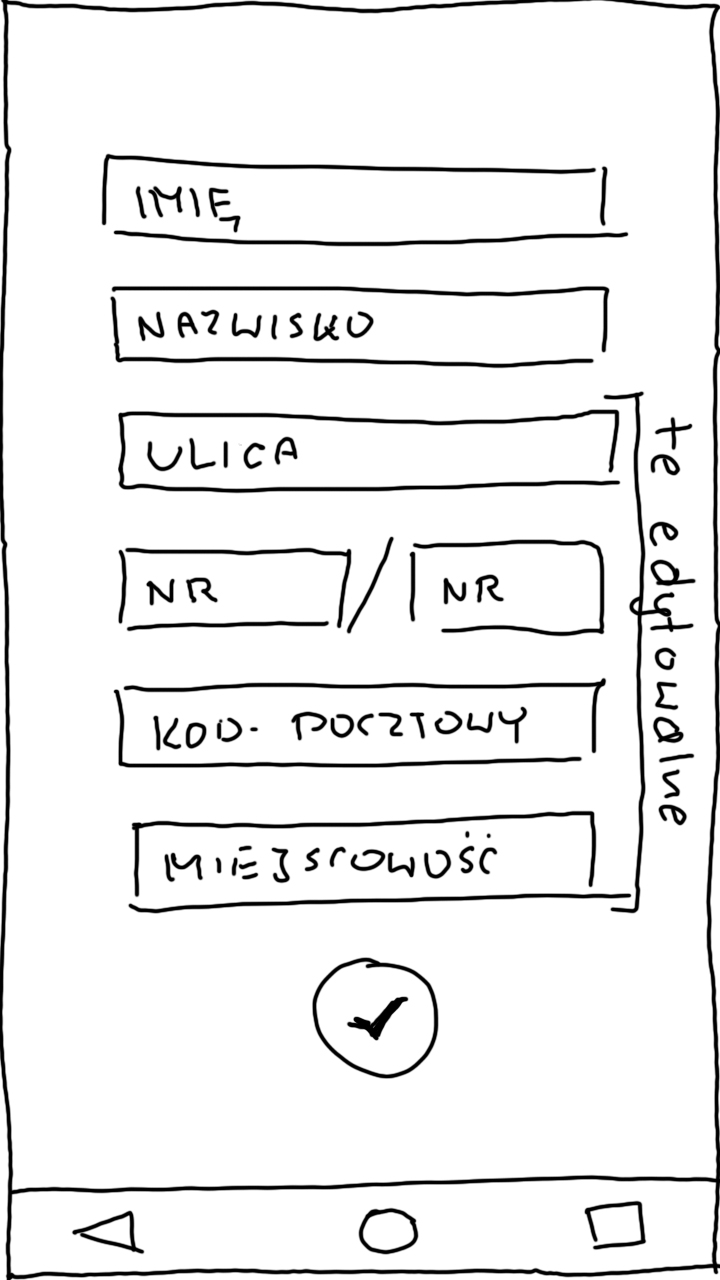
\includegraphics[width=.4\linewidth]{AplikacjaAndroid/Interfejs/ZmianaAdresu.jpg}
  \captionof{figure}{Zmiana adresu\\ (dla opiekuna)}
  \label{fig:test1}
\end{minipage}%
\begin{minipage}{.5\textwidth}
  \centering
  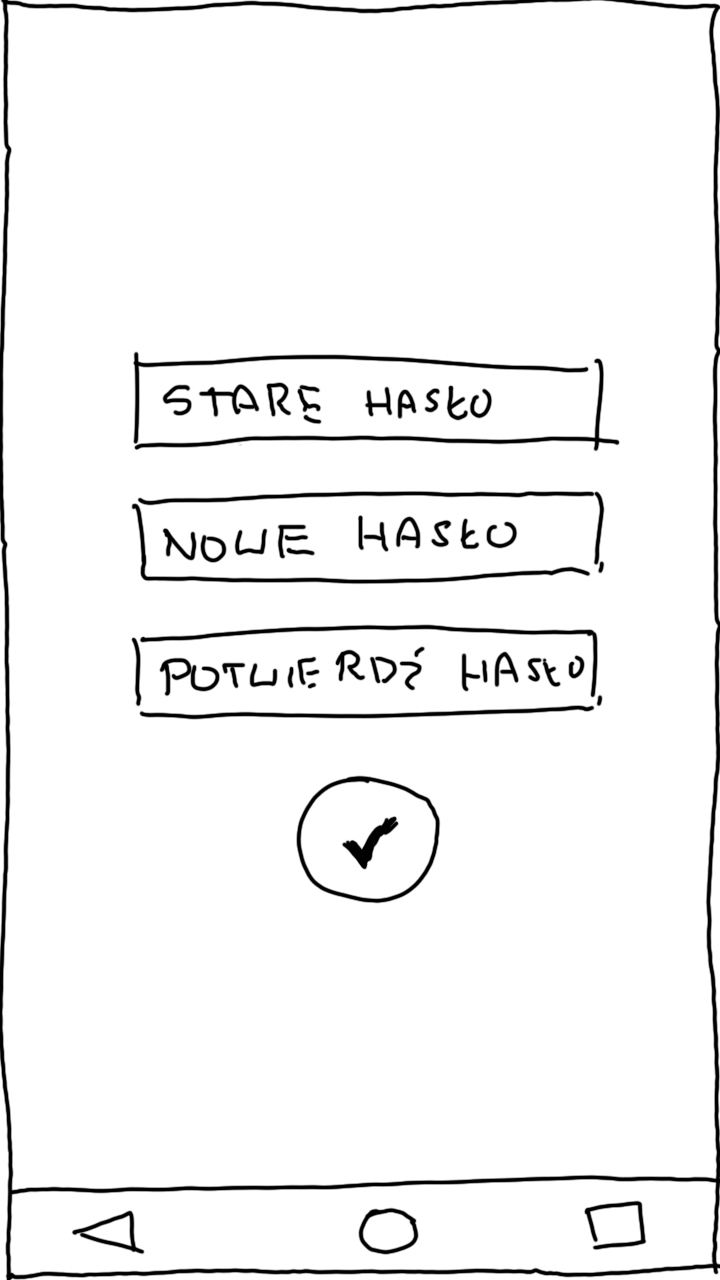
\includegraphics[width=.4\linewidth]{AplikacjaAndroid/Interfejs/ZmianaHasla.jpg}
  \captionof{figure}{Zmiana hasła}
  \label{fig:test2}
\end{minipage}
\end{figure}

\begin{figure}
\centering
\begin{minipage}{.5\textwidth}
  \centering
  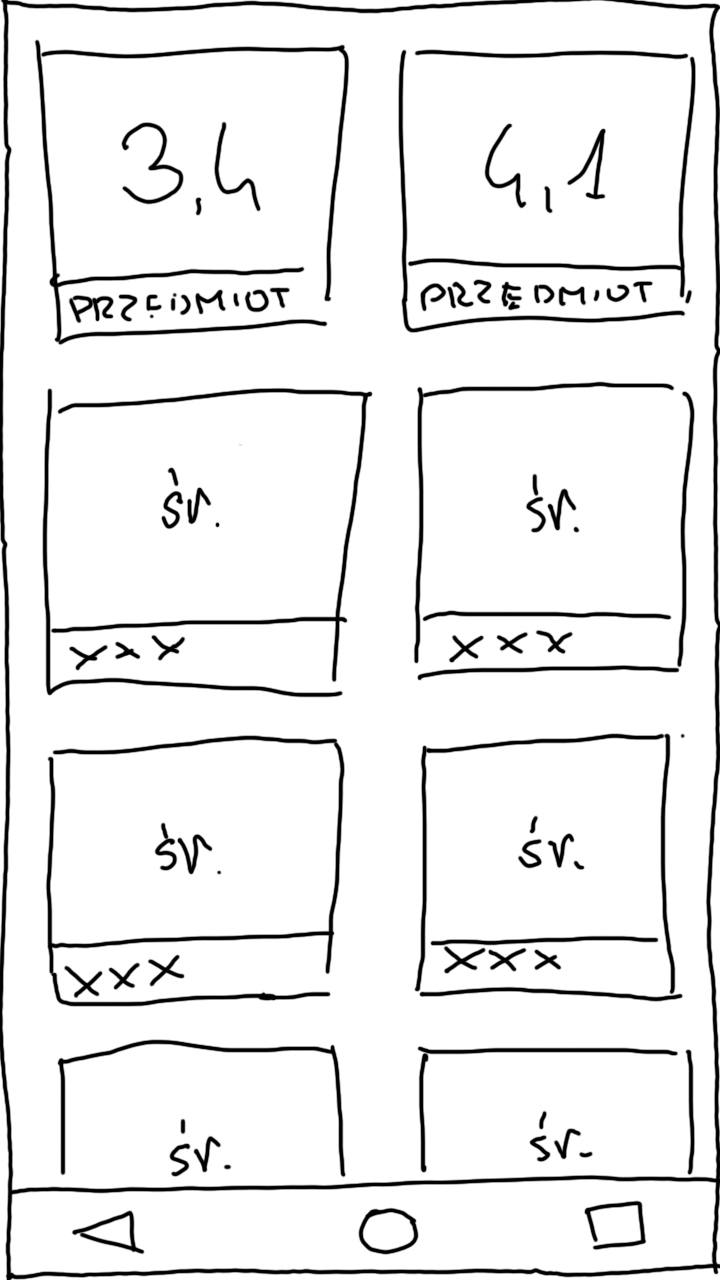
\includegraphics[width=.4\linewidth]{AplikacjaAndroid/Interfejs/Oceny1.jpg}
  \captionof{figure}{Widok główny ocen}
  \label{fig:test1}
\end{minipage}%
\begin{minipage}{.5\textwidth}
  \centering
  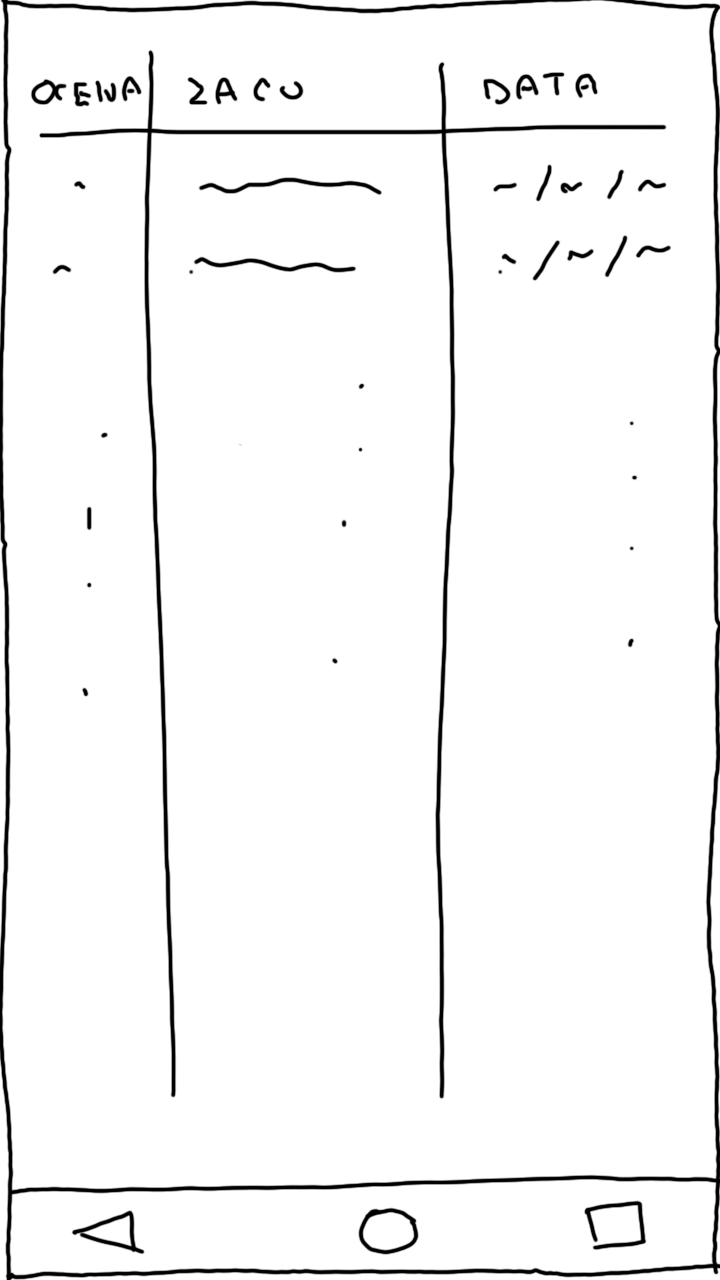
\includegraphics[width=.4\linewidth]{AplikacjaAndroid/Interfejs/Oceny2.jpg}
  \captionof{figure}{Widok ocen z przedmiotu}
  \label{fig:test2}
\end{minipage}
\end{figure}

\begin{figure}
\centering
\begin{minipage}{.5\textwidth}
  \centering
  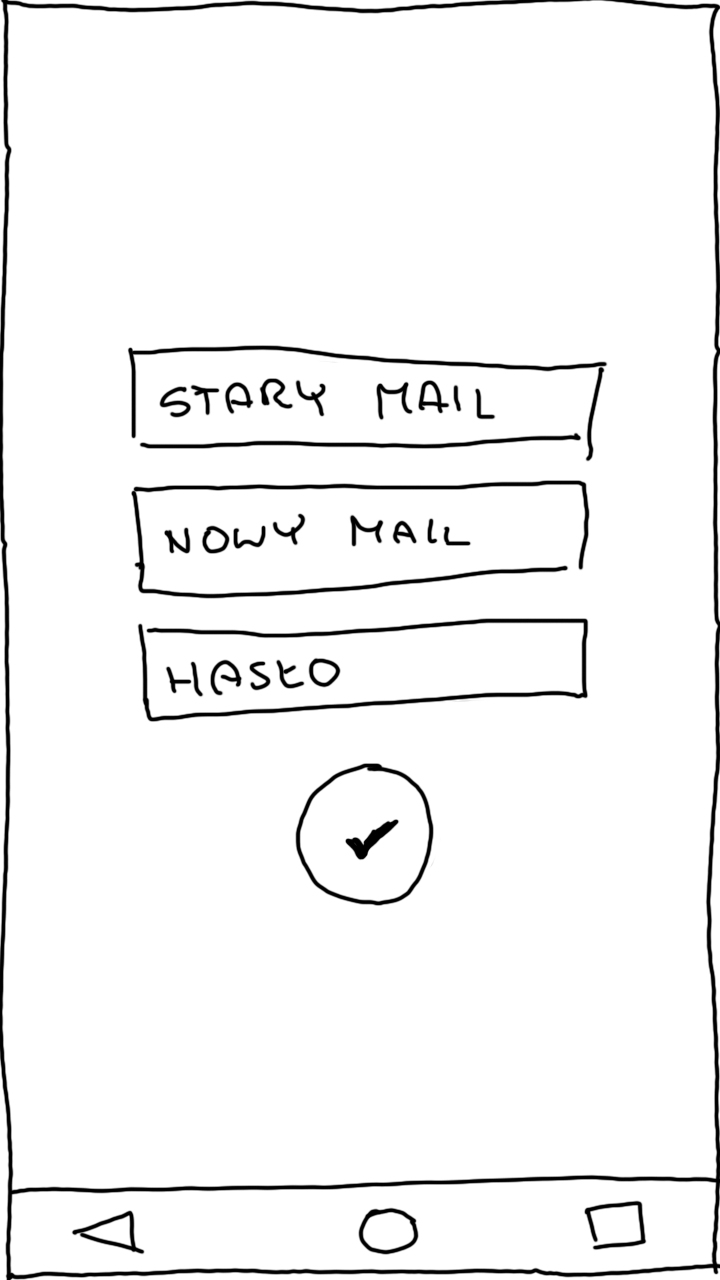
\includegraphics[width=.4\linewidth]{AplikacjaAndroid/Interfejs/ZmianaMaila.jpg}
  \captionof{figure}{Zmiana maila}
  \label{fig:test1}
\end{minipage}%
\begin{minipage}{.5\textwidth}
  \centering
  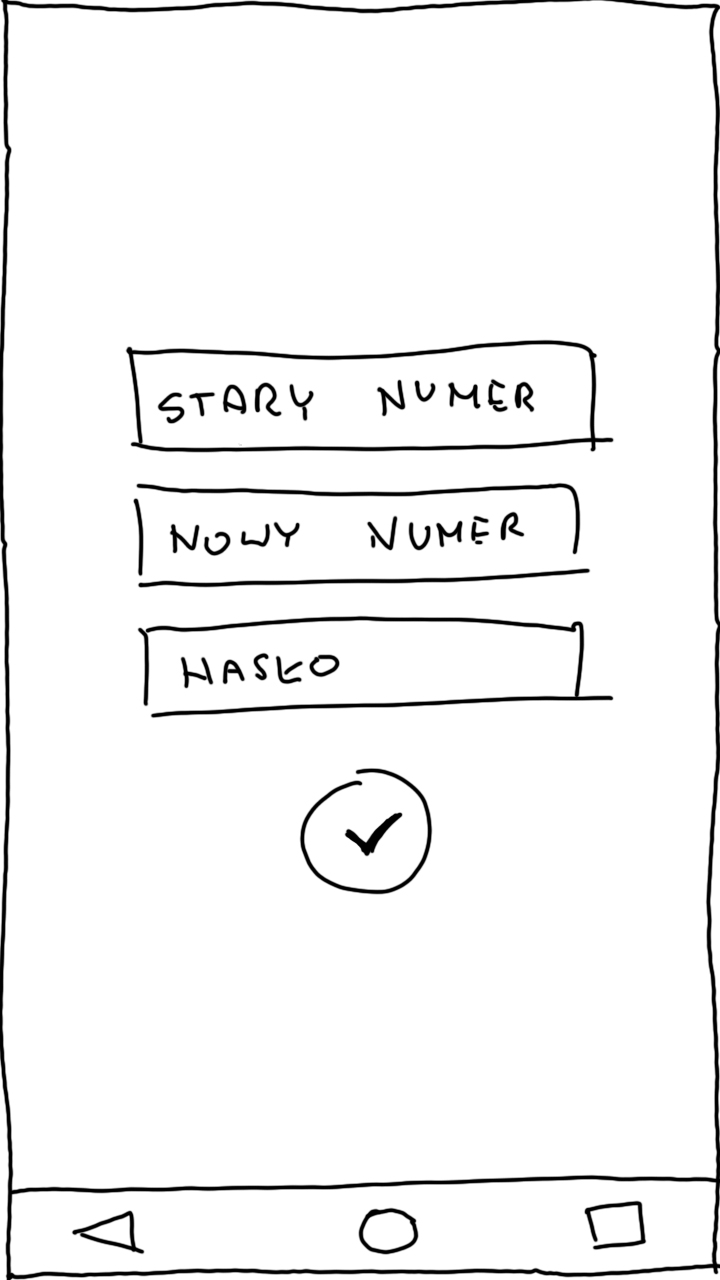
\includegraphics[width=.4\linewidth]{AplikacjaAndroid/Interfejs/ZmianaNumeru.jpg}
  \captionof{figure}{Zmiana numeru}
  \label{fig:test2}
\end{minipage}
\end{figure}

\begin{figure}
\centering
\begin{minipage}{.5\textwidth}
  \centering
  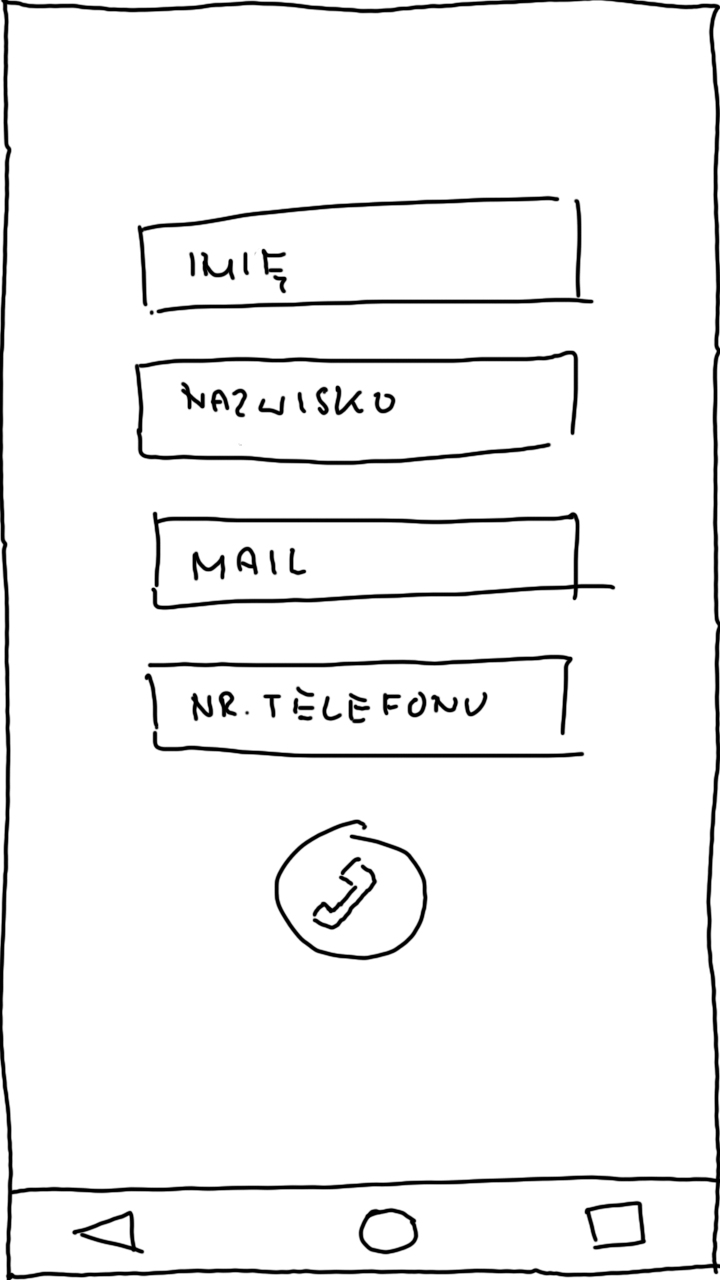
\includegraphics[width=.4\linewidth]{AplikacjaAndroid/Interfejs/Wychowawca.jpg}
  \captionof{figure}{Widok danych \\ wychowawcy}
  \label{fig:test1}
\end{minipage}%
\end{figure}

\subsection{Technologia}

Aplikacja kliencka działająca w systemie Android napisana w języku Java. Będzie łączyć się z serwerem za pomocą klasy HttpURLConnection. Wybór języka programowania na podstawie wspólnych preferencji oraz doświadczenia członków zespołu.

\section{Aplikacja webowa dla nauczyciela oraz administratora.}
\subsection{Technologia}
Aplikacja zostanie wykonana w technologii webowej, gdyż pozwala to na dostęp z każdego urządzenia posiadającego przeglądarkę internetową. \\
Skorzystamy z  bootstrapa, ponieważ są gotowe szablony dla stron administratorskich.
\subsection{Wymagania}
\begin{itemize}
\item Wymagania dla panelu administratora:
	\begin{itemize}
	\item tworzenie użytkowników oraz ich profili: nauczyciela, ucznia bądź opiekuna; 
	\item tworzenie klas i grup;
	\item przypisywanie: 
		\begin{itemize}
			\item nauczyciela do klasy jako wychowawcy;
			\item nauczyciela, grupy oraz przedmiotu do danej lekcji;
			\item uczniów do klas i grup;
		\end{itemize}
	\item przeglądanie ocen oraz danych 
	\end{itemize}
\item Wymagania dla panelu nauczyciela:
	\begin{itemize}
		\item zmiana danych własnych;
		\item przeglądanie, dodawanie oraz modyfikowanie ocen z własnych zajęć;
		\item przeglądanie danych dot. uczniów własnej klasy oraz ich opiekunów;
		\item przeglądanie ocen uczniów swojej klasy z innych zajęć;
	\end{itemize}
\end{itemize}
\subsection{Interfejs}
Dwa różne interfejsy:
\begin{itemize}
	\item dla nauczyciela,
	\item dla administratora.
\end{itemize}
Oba opierają się na idei nawigatora po lewej stronie.
\subsubsection{Interfejs nauczyciela}
Interfejs nauczyciela powinien posiadać zakładki:
\begin{itemize}
	\item Zajęcia - dostęp do zajęć prowadzonych przez danego nauczyciela. Po kliknięciu na daną lekcję odsyłany jest on do strony z tabelą z ocenami. 
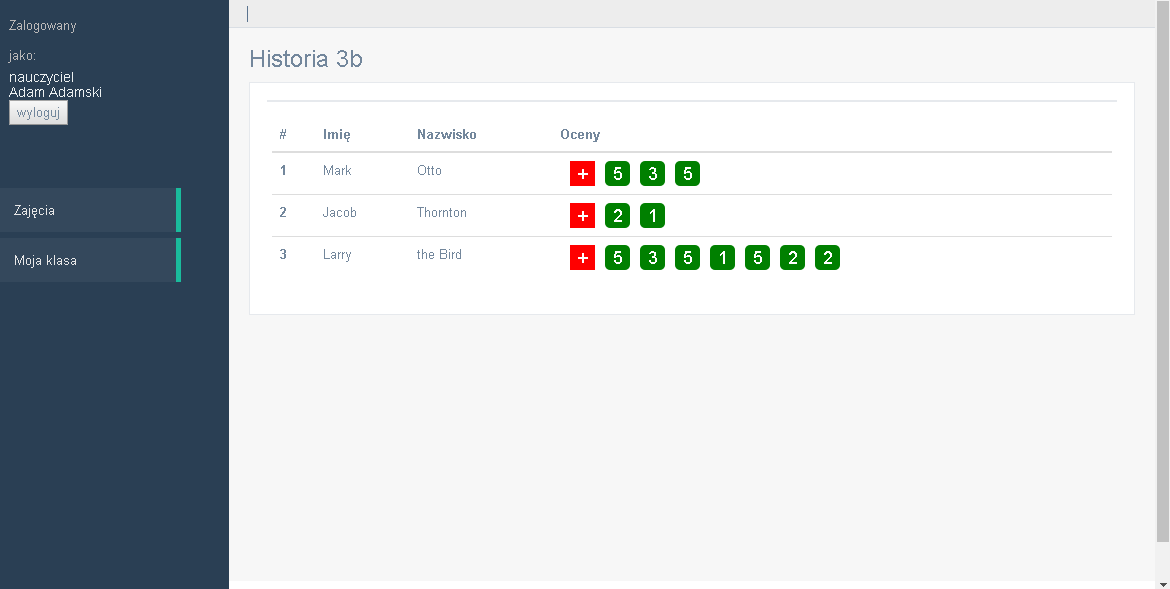
\includegraphics[scale=0.4]{screeny/nauczyciel.png}
	\item Moja klasa - klasa, której wychowawcą jest dany nauczyciel - jeżeli nie jest wychowawcą żadnej klasy to zakładka ta nie pojawia się. Tutaj nauczyciel ma prawo przejrzeć swoich uczniów oraz ich oceny z poszczególnych zajęć. \\
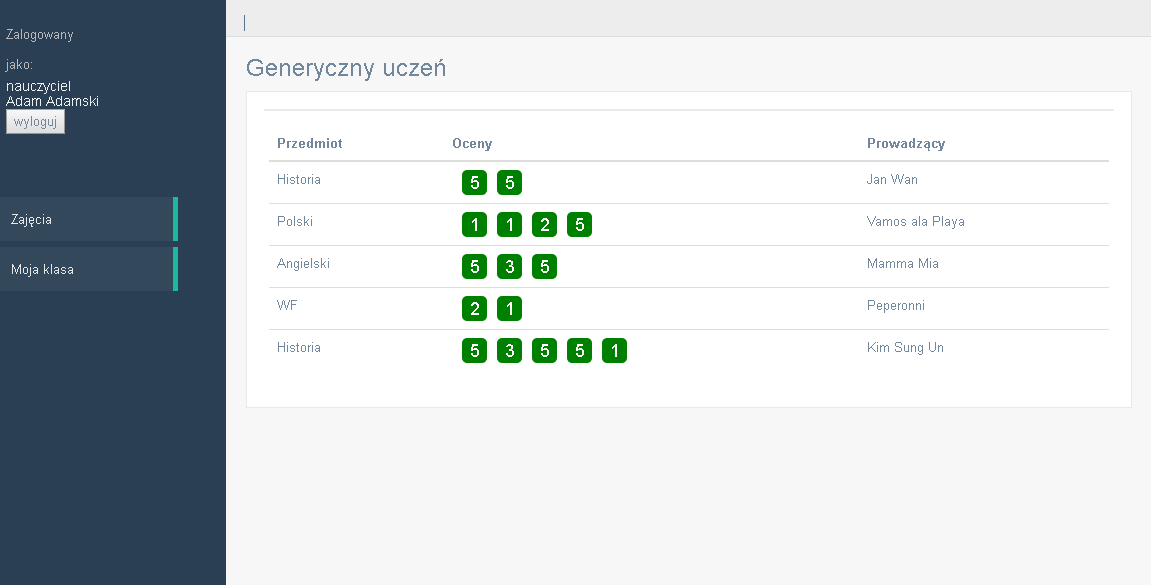
\includegraphics[scale=0.4]{screeny/Oceny.png}
\end{itemize}

\subsubsection{Interfejs administratora}
Administrator ma dostęp w pasku nawigacyjnym do listy użytkowników jak i osób, klas i grup. \\
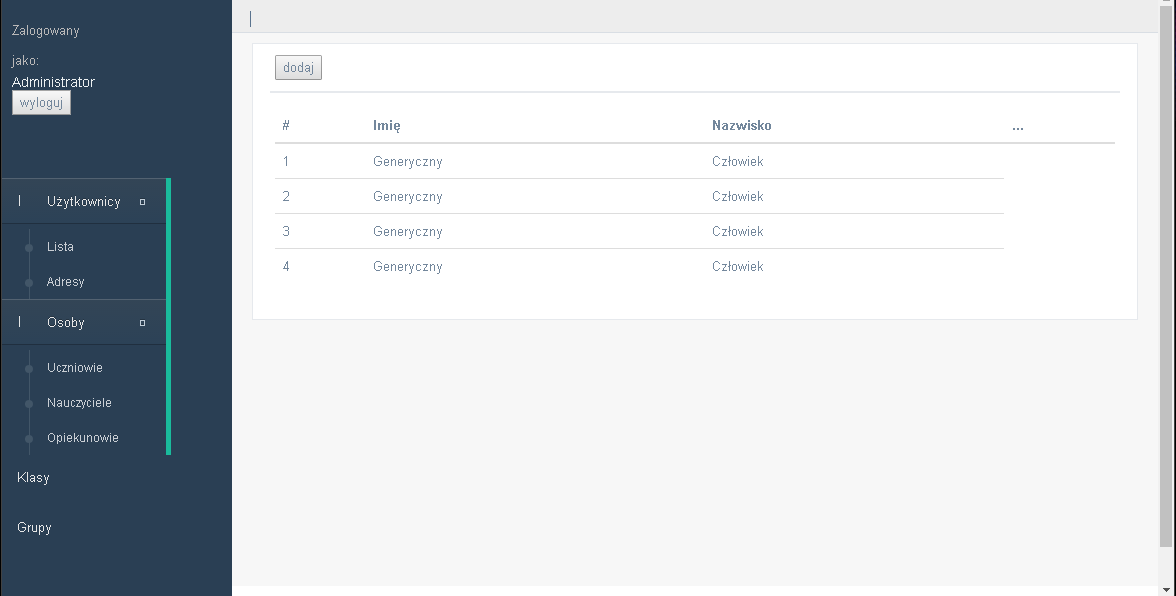
\includegraphics[scale=0.4]{screeny/admin.png}


\section{Baza danych}

\subsection{Technologia}
Baza danych została napisana w MySQL. Jest to ogólnodostępny system, umożliwiający zarządzanie relacyjnymi bazami danych. Zdecydowaliśmy się na niego, ponieważ jest dostępny na wielu platformach, darmowy i posiada rozbudowaną dokumentację. 

\subsection{Narzędzia}
Do stworzenia i zarządzania bazą danych wykorzystaliśmy panel administratorski do baz danych na serwerze \textit{home.pl}. 

Zapytania oraz połączenie z aplikacją zostały napisane w \textit{IntelliJ}, a do podglądu stworzonych zapytań wykorzystaliśmy dodatek do Google Chrome - aplikację \textit{Postman}. 

\subsection{Diagram}
\begin{center}
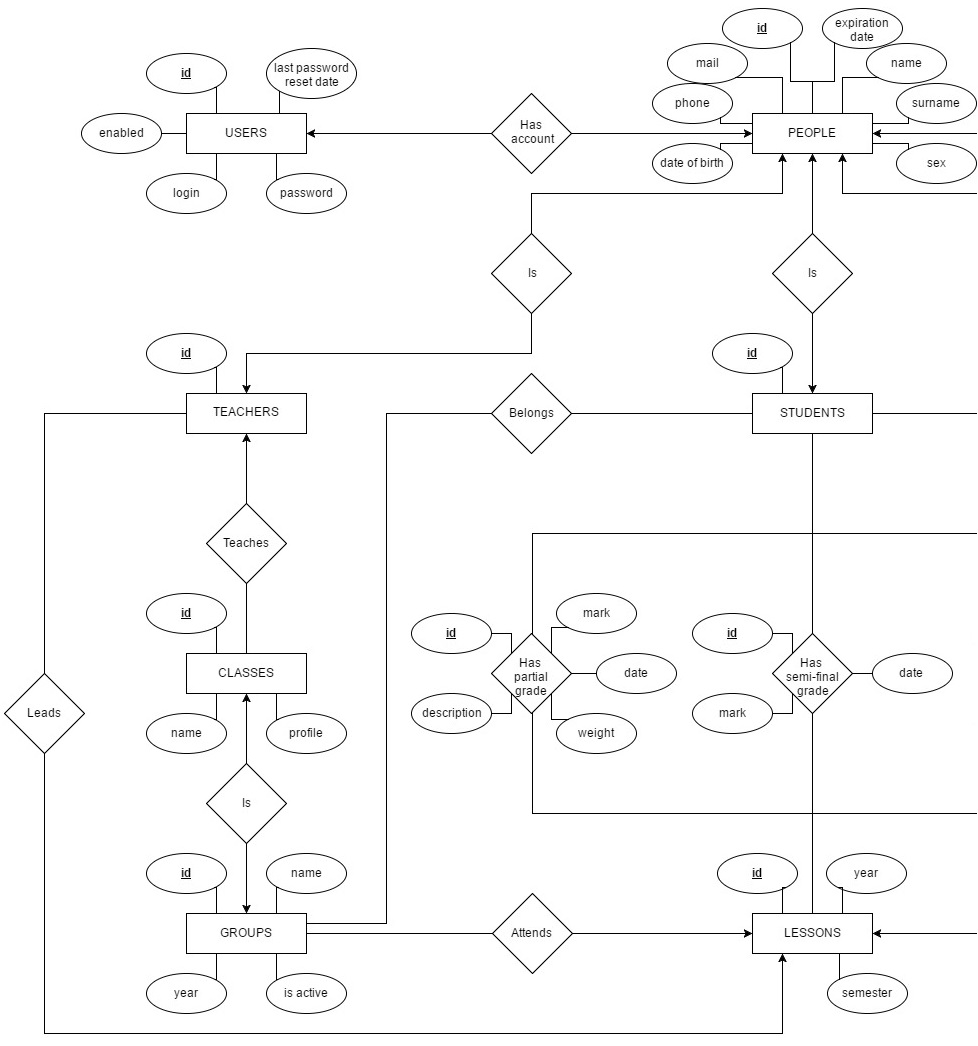
\includegraphics[scale=0.5]{screeny/diagram1.jpg}
\end{center}

\begin{center}
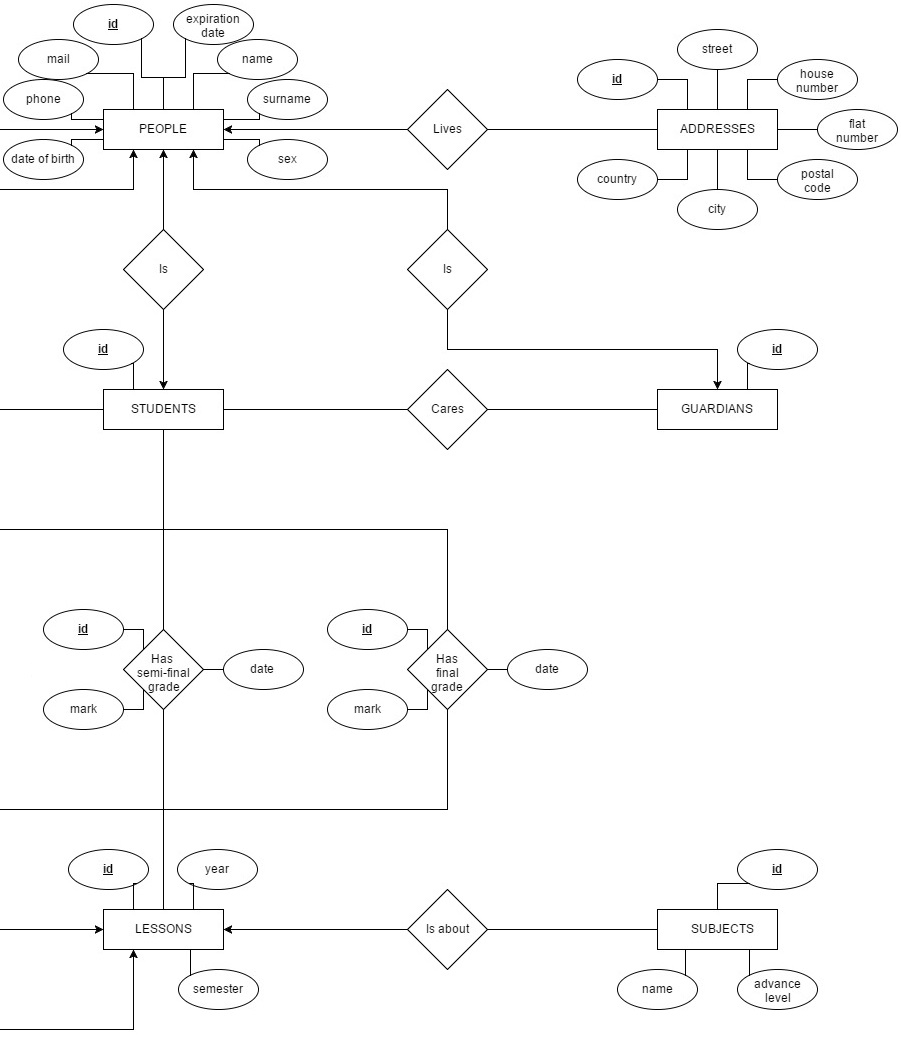
\includegraphics[scale=0.5]{screeny/diagram2.jpg}
\end{center}


Przedstawione diagramy zostały przygotowane z użyciem darmowego edytora \textit{draw.io}. 


\subsection{Relacyjny model bazy danych}
\begin{center}
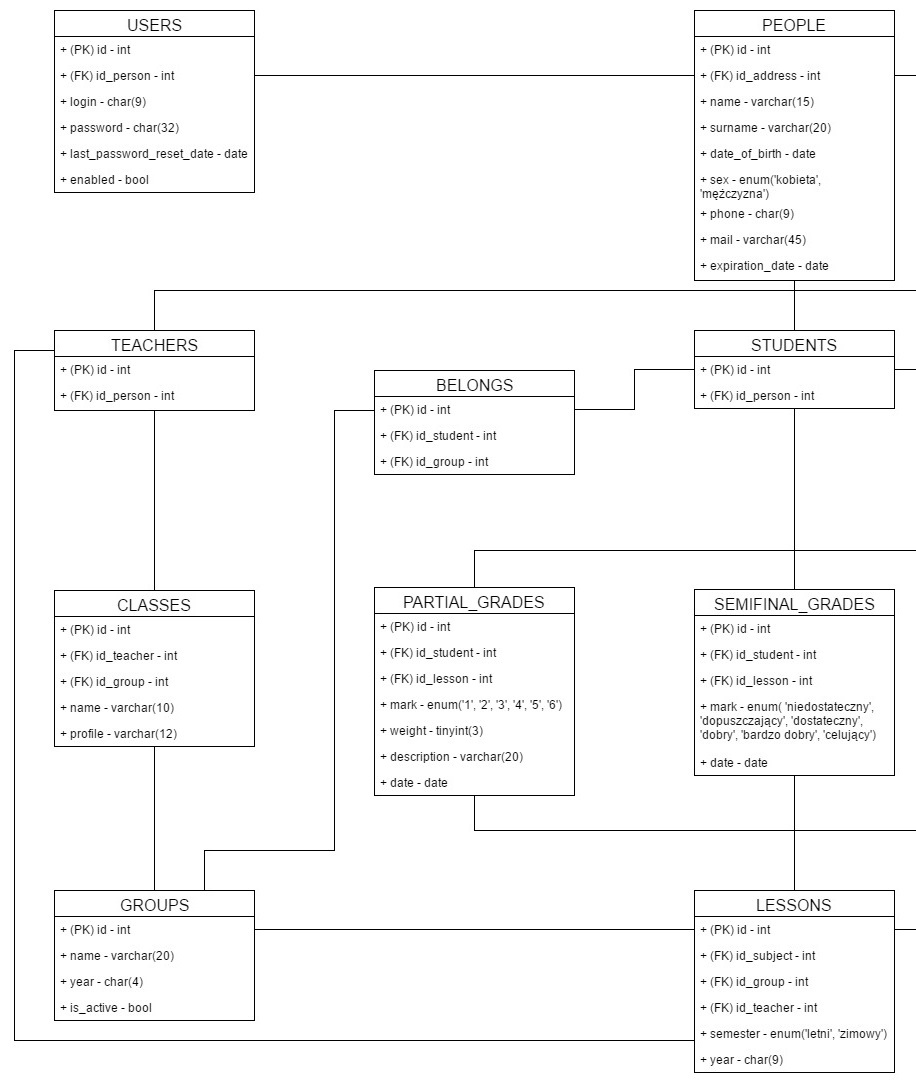
\includegraphics[scale=0.5]{screeny/relational1.jpg}
\end{center}

\begin{center}
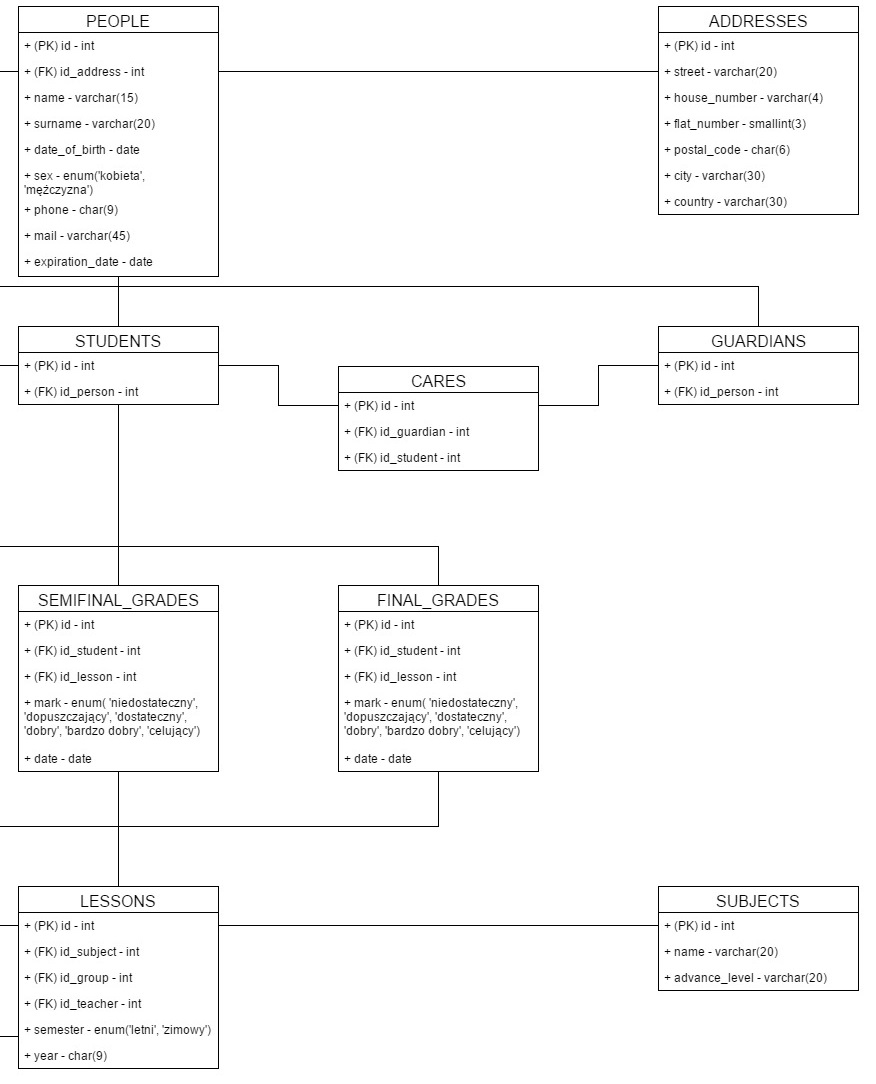
\includegraphics[scale=0.5]{screeny/relational2.jpg}
\end{center}

\subsection{Dane, o które pytamy}

\begin{enumerate}
	\item W trakcie logowania użytkownika:
	\begin{itemize}
		\item czy podany login jest w bazie
		\item czy dla podanego loginu użytkownik wprowadził poprawne hasło
		\item kim jest osoba logująca – admin, nauczyciel, uczeń, opiekun
	\end{itemize}	
	\item W trakcie tworzenia użytkownika przez admina:
	\begin{itemize}
		\item dodawanie nowego użytkownika, wprowadzenie nowego adresu i danych osobowych
		\item przypisanie użytkownika do klasy/zajęć/dziecka/opiekuna….
	\end{itemize}	
	\item Zalogowany nauczyciel:
	\begin{itemize}
		\item lista zajęć które prowadzi (przedmiot, grupa)
		\item lista uczniów, którzy są w danej grupie
		\item dodawanie ocen (uczniowi z konkretnych zajęć, data, opis, waga, stopień)
		\item po dodaniu oceny aktualizacja średniej ważonej ocen
		\item edycja ocen/usuwanie
	\end{itemize}	
	\item Zalogowany opiekun/uczeń:
	\begin{itemize}
		\item lista zajęć na które uczęszcza uczeń (nazwa przedmiotu, prowadzący)
		\item lista ocen z poszczególnych zajęć (data, opis, ocena)
		\item średnia ważona obliczona na podstawie wystawionych dotychczas stopni
		\item dane wychowawcy klasy, do której należy uczeń
		\item dla opiekuna lista jego podopiecznych
	\end{itemize}	
	\item Zalogowany użytkownik:
	\begin{itemize}
		\item wgląd do swoich danych z możliwością edycji (adres, mail, telefon, ...)
	\end{itemize}	
\end{enumerate}

\section{Serwer}

\subsection{Technologia}
Usługa została napisana w języku Java, framework Spring Boot. Użyliśmy Spring Boota ze względu na dobrą dokumentacje oraz stosunkowo krótki czas konfiguracji. System logowania oparty jest na tokenach w standardzie JSON Web Token, jest to standard wolnego dostępu, dobrze udokumentowany.

\subsection{Narzędzia}

Korzystamy ze środowiska IntelliJ do programowania serwisu. Do komunikacji z serwerem wykorzystujemy wtyczkę do przeglądarki Google Chrome - Postman.

\subsection{Opis endpointów}

Z aplikacją serwerową można komunikować się poprzez restowe API.

\subsubsection{Logowanie}

\begin{enumerate}

	\item "/auth" \\
	Opis: Generuje token do autoryzacji zapytań do serwisu na podstawie logina i hasła użytkownika.\\
		Metoda: POST\\
		Body: "\{"login":"login", "password":"password"\}"\\ (klasa JwtCredentials)
		Odpowiedź: \{"status":"status odpowiedzi", "token":"token"\}\\
		(klasa JwtAuthenticationResponse)
	
\end{enumerate}

\subsubsection{Grupy}

\begin{enumerate}
	\item 
	{\renewcommand{\arraystretch}{1.5}
	\begin{tabular}[t]{p{3cm} p{15cm}}
	\multicolumn{2}{l}{"/Groups/teacher/myGroups":} \\
	Opis: &  Lista grup, w których użytkownik prowadzi zajęcia. \newline Id użytkownika wyciągane z tokenu. \\
	Metoda: & GET \\
	Header: & \{"Authorization":"wygenerowany token"\} \\
	Odpowiedź: & \{"status":"status odpowiedzi",\newline "groups":[(lista grup)]\} \\
	Przykładowa \newline odpowiedź: & 			\{"status": "ok",\newline "groups": [\newline \{ "id": 1,\newline "name": "IB",\newline "year": null,\newline "active": false\},\newline \ldots
	\end{tabular}}
	
	\item 
	{\renewcommand{\arraystretch}{1.5}
	\begin{tabular}[t]{p{3cm} p{15cm}}
	\multicolumn{2}{l}{"/Groups/attendingStudents/{idGroup}":} \\
	Opis: &  Lista uczniów należących do danej grupy. \\
	Metoda: & GET \\
	Header: & \{"Authorization":"wygenerowany token"\} \\
	Odpowiedź: & \{"status":"status odpowiedzi",\newline "people":[(lista osób)]\}
	\end{tabular}}
	
	\item 
	{\renewcommand{\arraystretch}{1.5}
	\begin{tabular}[t]{p{3cm} p{15cm}}
	\multicolumn{2}{l}{"/Groups/myClass":} \\
	Opis: &  Klasa, do której należy uczeń. \newline Id użytkownika wyciągane z tokenu.\\
	Metoda: & GET \\
	Header: & \{"Authorization":"wygenerowany token"\} \\
	Odpowiedź: & \{"status":"status odpowiedzi",\newline "groupClass":\{(klasa\}\} \\
	Przykładowa \newline odpowiedź: & 			\{"status": "ok",\newline "groupClass": [\newline \{ "name": "IVA",\newline "profile": null,\newline "idTutor": 7,\newline "tutorName": "Andrzej", \newline "tutorSurname": "Maciejewski"\},\newline \ldots
	\end{tabular}}
	
	\item 
	{\renewcommand{\arraystretch}{1.5}
	\begin{tabular}[t]{p{3cm} p{15cm}}
	\multicolumn{2}{l}{"/Groups/userClass/userId={userId}":} \\
	Opis: &  Klasa, do której należy podany użytkownik. \\
	Metoda: & GET \\
	Header: & \{"Authorization":"wygenerowany token"\} \\
	Odpowiedź: & \{"status":"status odpowiedzi",\newline "groupClass":\{(klasa)\}\}
	\end{tabular}}
\end{enumerate}


\subsubsection{Oceny}

\begin{enumerate}
	\item 
	{\renewcommand{\arraystretch}{1.5}
	\begin{tabular}[t]{p{3cm} p{15cm}}
	\multicolumn{2}{l}{"/Grades/myGrades":} \\
	Opis: &  Posortowana (by id lesson) lista ocen zalogowanego użytkownika. \newline Id użytkownika wyciągane z tokenu. \\
	Metoda: & GET \\
	Header: & \{"Authorization":"wygenerowany token"\} \\
	Odpowiedź: & \{"status":"status odpowiedzi",\newline "grades":[(tablica ocen)]\} \\
	Przykładowa \newline odpowiedź: & 			\{"status": "ok",\newline "grades": [\newline \{ "id": 1,\newline "mark": "5+",\newline "weight": 1,\newline "description": null,\newline "date": "2016-10-19",\newline "idStudent": 5,\newline "idLesson": 4,\newline "subjectName": "język polski"\},\newline \ldots
	\end{tabular}}
	
	\item 
	{\renewcommand{\arraystretch}{1.5}
	\begin{tabular}[t]{p{3cm} p{15cm}}
	\multicolumn{2}{l}{"/Grades/myGrades/{idLesson}":} \\
	Opis: &  Lista ocen zalogowanego użytkownika z danej lekcji.\newline Id użytkownika wyciągane z tokenu. \\
	Metoda: & GET \\
	Header: & \{"Authorization":"wygenerowany token"\} \\
	Odpowiedź: & \{"status":"status odpowiedzi",\newline "grades":[(tablica ocen)]\}
	\end{tabular}}
	
	\item 
	{\renewcommand{\arraystretch}{1.5}
	\begin{tabular}[t]{p{3cm} p{15cm}}
	\multicolumn{2}{l}{"/userGrades/{idUser}":} \\
	Opis: &  Lista ocen dla użytkownika o podanym id. \\
	Metoda: & GET \\
	Header: & \{"Authorization":"wygenerowany token"\} \\
	Odpowiedź: & \{"status":"status odpowiedzi",\newline "grades":[(tablica ocen)]\}
	\end{tabular}}
	
	\item 
	{\renewcommand{\arraystretch}{1.5}
	\begin{tabular}[t]{p{3cm} p{15cm}}
	\multicolumn{2}{l}{"/userGrades/{idUser}/lesson/{idLesson}":} \\
	Opis: &  Lista ocen dla użytkownika o podanym id z danej lekcji. \\
	Metoda: & GET \\
	Header: & \{"Authorization":"wygenerowany token"\} \\
	Odpowiedź: & \{"status":"status odpowiedzi",\newline "grades":[(tablica ocen)]\}
	\end{tabular}}
\end{enumerate}

\subsection{Opis usługi}

Do aplikacji można się logować jako uczeń ('STUDENT'), opiekun ('GUARDIAN'), nauczyciel ('TEACHER'). Każda z ról ma różny dostęp do API, dostęp do endopintu jest ustawiany za pomocą adnotacji @PreAuthorize("hasRole('TEACHER')").


\end{document}
